\documentclass[conference]{IEEEtran}
\usepackage{cite}
\usepackage{amsmath,amssymb,amsfonts}
\usepackage{algorithmic}
\usepackage{graphicx}
\usepackage{textcomp}
\usepackage{comment}
\renewcommand{\refname}{Referencias}
\renewcommand{\tablename}{TABLA}


\def\BibTeX{{\rm B\kern-.05em{\sc i\kern-.025em b}\kern-.08em
    T\kern-.1667em\lower.7ex\hbox{E}\kern-.125emX}}
\begin{document}
\title{Predicción de complicaciones durante la hospitalización del paciente de infarto de miocardio}


\author{\IEEEauthorblockN{Juan Acostupa}
\IEEEauthorblockA{\textit{Dpto. de Ing. Informática PUCP} \\
Lima, Perú\\
a20244906@pucp.edu.pe}
\and
\IEEEauthorblockN{Breno Muñoz}
\IEEEauthorblockA{\textit{Dpto. de Ing. Informática PUCP} \\
Lima, Perú\\
a20162955@pucp.edu.pe}
\and
\IEEEauthorblockN{Ronny Huerta}
\IEEEauthorblockA{\textit{Dpto. de Ing. Informática PUCP} \\
Lima, Perú \\
a20184255@pucp.edu.pe}
}

\maketitle

\section{Introducción}
El ataque al miocardio es una de las complicaciones de salud que causan mas muertes a nivel mundial, en el Perú por ejemplo, mas de 4 mil personas mueren al año debido a esta emergencia médica \cite{b2}. Las causas que lo originan son diversas como: enfermedad de las arterias coronarias, acumulación de colesterol, artereoesclerosis, coágulos de sangre formados en las arterias, atero-trombosis, la edad, el sedentarismo, y una alimentación desbalanceada. Sin embargo, se ha estudiado que esta enfermedad cardiovascular tiene patrones los cuales puedes ser usados para su análisis mediante  el uso de una gran cantidad de datos recogidos de pacientes como en \cite{b1}, para su aplicación de modelos de aprendizaje automático. 

El presente estudio se focaliza en el tratamiento de los datos de dos problemas: el primero, en la predicción de las complicaciones que pueda tener el paciente basado en la información recolectada al momento de su internamiento, y el segundo problema de la predicción de las complicaciones luego de un periodo de tres días de internamiento en el hospital.

El presente informe se organiza de la siguiente manera: en primer lugar, se describe una introducción general a la problemática (sección I) junto con el objetivo principal a abordar en el presente trabajo; en la segunda parte (sección II) se hace una breve síntesis del estado del arte con artículos científicos usando los mismos datos del presente proyecto y con otros diferentes pero con alternativas de solución en relación al problema mencionado; en la tercera parte (sección III) se explica sobre el diseño del experimento, en el cual se ha hace una descripción detallada del conjunto de datos y la metodología a usar para el abordaje del presente proyecto.

\section{Estado del arte}
Existen múltiples trabajos que tratan sobre diferentes aspectos relacionados a la utilización de diferentes algoritmos de aprendizaje automático y la importancia del rol que juegan estos métodos en la mejora del diagnóstico y prevención de complicaciones. \textit{Quer et. al.} \cite{e1} hace un énfasis especial en el rol que juegan el personal médico, en especial los cardiólogos. Asimismo, \textit{Van den Eynde et. al.} \cite{e2} hacen mención de un número de ejemplos exitosos de técnicas de inteligencia artificial en casos de cardiología clínica, mientras que \textit{Sevakula et. al.} \cite{e3} hacen un estudio sobre nuevos casos que se le pueden dar a estas técnicas, además de las limitaciones que estas tienen. Finalmente, \textit{Benzakour et. al.} \cite{zz} hace un estudio extenso de los conjuntos de datos publicados sobre diferentes tipos de enfermedades cardiovasculares, encontrando 39 conjuntos de datos diferentes. Entre ellos, el dataset objeto de estudio del presente trabajo.

El dataset Myocardial Infarction Complications Database se ha utilizado previamente para predecir complicaciones en pacientes que han sufrido infarto del miocardio. A continuación se resumen las metodologías respecto del tratamiento de los datos y los modelos de clasificación sobre estos mismos datos y sobre otras bases de datos \cite{bp}. 

\subsubsection{Preprocesamiento}
Respecto del preprocesamiento de los datos, algunos autores coinciden en tratar los datos faltantes eliminando aquellas variables cuyos faltos exceden un límite porcentual máximo. En cambio, otros utilizan técnicas de reducción de la dimensionalidad\cite{bp} como el Análisis de Componentes Principales (PCA) y el catPCA. Teóricamente, este último está pensado para mantener la máxima correlación entre las variables cuando se tienen salidas con datos de tipo categórico \cite{b1}. Otros autores han tomado la alternativa de utilizar técnicas innovadoras para intentar imputar valores nulos \cite{ll}. Adicionalmente, se observa que se ha intentado abordar el desbalance de clases utilizando métodos conjuntos de sobre o sub muestreo y métricas sensibles a la clase minoritaria \cite{by}\cite{ll}

\subsubsection{Clasificadores}
 En esta categoría se han implemenado modelos como Regresión Logística\cite{bx}\cite{bz}, Redes Neuronales \cite{bx}\cite{bz}\cite{ll}\cite{bp}, XGBOOST\cite{bz}\cite{bp}, Máquina de Vectores de Soporte (SVM)\cite{bz}, Bosques Aleatorios\cite{bz} y k-Vecindarios Más Cercanos\cite{b?}\cite{by}. Esto puede deberse a que los modelos son adecuados para la clasificación de variables del tipo categórico. En general, se observa un éxito entre moderado y alto el cual puede depender de las variables que se eligen para realizar la predicción, donde individualmente se ha logrado sobrepasar métricas en más de 91\%.

\section{Diseño del Experimento}
\subsection{Descripción del conjunto de datos}\label{EDA}
El conjunto de datos contiene información sobre pacientes que han sufrido un infarto al miocardio y complicaciones asociadas a esta afección. De acuerdo a \cite{b1}, este conjunto de datos contiene registros recolectados por el Hospital Clínico Interdistrital de Krasnoyarsk, en Rusia, durante los años 1992-1995. 
\subsubsection{Número y Tipo de variables}\label{nvar}
El conjunto de datos consta de dos partes. La primera contiene variables que se pueden considerar "de entrenamiento", conformando un total de 110. Estas variables incluyen:
\begin{itemize}
    \item 78 variables binarias.
    \item 16 variables categóricas.
    \item 9 variables numéricas discretas.
    \item 7 variables numéricas contínuas.
\end{itemize}

Algunas de las características más relevantes contienen información demográfica, antecedentes médicos (arritmias, insuficiencias cardiacas, entre otros), factores de riesgo cardiovascular e información de los primeros días de seguimiento al paciente post-infarto.

La segunda parte del conjunto de datos consta de variables que contienen información de diferentes tipos de complicaciones relacionadas a infarto en el miocardio. Estas variables se pueden considerar como "objetivos", y son un total de 12, siendo estas:
\begin{itemize}
\item 11 variables binarias.
\item 1 variable categórica.
\end{itemize}

\subsubsection{Número de muestras}\label{nmue}
El conjunto de datos contiene un total de 1700 registros. No existe una separación entre conjunto de entrenamiento y conjunto de prueba, pero esta separación es necesaria para cumplir con el objetivo del presente análisis, por lo que se va a realizar siguiendo la estrategia utilizada en la sección de metodología.

\subsubsection{Número de muestras por clase}\label{nmue}
Este conjunto de datos contiene un total de 12 variables que se pueden considerar como objetivo, de las cuales 11 son binarias. La distribución de clases de cada una de estas variables binarias es:

\begin{table}[ht]
\centering
\caption{Número de muestras por variable binaria}
\begin{tabular}{l|r|r}
\textbf{Variable} & \textbf{Clase = 0} & \textbf{Clase = 1} \\
\hline
\rule{0pt}{3ex}
    FIBR\_PREDS & 1530 & 170 \\
    PREDS\_TAH & 1680 & 20 \\
    JELUD\_TAH & 1658 & 42 \\
    FIBR\_JELUD & 1629 & 71 \\
    A\_V\_BLOK & 1643 & 57 \\
    OTEK\_LANC & 1541 & 159 \\
    RAZRIV & 1646 & 54 \\
    DRESSLER & 1625 & 75 \\
    ZSN & 1306 & 394 \\
    REC\_IM & 1541 & 159 \\
    P\_IM\_STEN & 1552 & 148 \\
\end{tabular}
\label{tab:num_samples}
\end{table}

Mientras tanto, la variable categórica tiene la siguiente distribución:

\begin{table}[ht]
\centering
\caption{Distribución de clases de la variable categórica LET\_IS}
\begin{tabular}{c|c}

\textbf{Valor de LET\_IS} & \textbf{Frecuencia} \\
\hline
    \rule{0pt}{3ex}
    0 & 1429 \\
    1 & 110 \\
    3 & 54 \\
    7 & 27 \\
    6 & 27 \\
    4 & 23 \\
    2 & 18 \\
    5 & 12 \\

\end{tabular}
\label{tab:let_is_dist}
\end{table}

Por un lado, las variables de predicción del dataset sufren del problema del desbalance. Generalmente, se observa una proporción de alrededor 1 a 9 entre casos positivos y negativos (Tabla \ref{tab:num_samples}), respectivamente. En base a esto, será necesario tomar en cuenta el problema de el desbalance de clases durante el entrenamiento para evitar el sesgo hacia la clase negativa. 

Por otro lado, las variables de entrada contienen una gran cantidad de valores faltantes. De las 110 variables de entrada, 11 de ellas presentan al menos 20\% de valores faltantes (Tabla \ref{above_20_misssing_values_from_input}).

\begin{table}[ht!]
\centering
\caption{Variables con más de 20\% de valores faltantes}
    \begin{tabular}{l|c}
    \textbf{Variable} & \textbf{Porcentaje de valores faltantes} \\
    \hline
    \rule{0pt}{3ex}
    IBS\_NASL     & 95.7 \\
    S\_AD\_KBRIG   & 63.2 \\
    D\_AD\_KBRIG   & 63.2 \\
    GIPO\_K       & 21.7 \\
    K\_BLOOD      & 21.8 \\
    GIPER\_NA     & 22.0 \\
    NA\_BLOOD     & 22.0 \\
    KFK\_BLOOD    & 99.7 \\
    NA\_KB        & 38.6 \\ 
    NOT\_NA\_KB    & 40.3 \\
    LID\_KB       & 39.8 \\
    \end{tabular}
\label{above_20_misssing_values_from_input}
\end{table}

\subsubsection{Estadística descriptiva}\label{edes}
Este conjunto de datos contiene información de 111 variables descriptivas, que brindan información detallada de varios aspectos relacionados al paciente. Para poder obtener información del conjunto de datos, se ha optado por utilizar un algoritmo de clustering sobre la base de correlaciones, con lo cual, se han agrupado las 111 variables en 5 categorías distintas. La figura \ref{fig:fig1} muestra una representación visual del método de clustering basado en la correlación entre variables utilizado.

De acuerdo a las variables agrupadas en cada clúster, se puede interpretar a grandes razgos a cada cluster de la siguiente manera:

\begin{itemize}
    \item Clúster \#1: (38 variables) Características generales del paciente, antecedentes médicos, hallazgos electrocardiográficos y manejo inicial en la unidad de cuidados intensivos.
    \item Clúster \#2: (8 variables) Seguimiento de los síntomas y manejo del dolor en los primeros días de hospitalización.
    \item Cluster \#3: (34 variables) Factores de riesgo cardiovascular, hallazgos clínicos y de laboratorio al ingreso, y manejo terapéutico inicial. 
    \item Clúster \#4: (27 variables) Antecedentes de arritmias e insuficiencia cardíaca, y hallazgos electrocardiográficos y clínicos relacionados al ingreso.
    \item Clúster \#5: (4 variables) Niveles séricos de electrolitos clave (potasio y sodio).
\end{itemize}

\begin{figure}[htbp!]
  \centering
  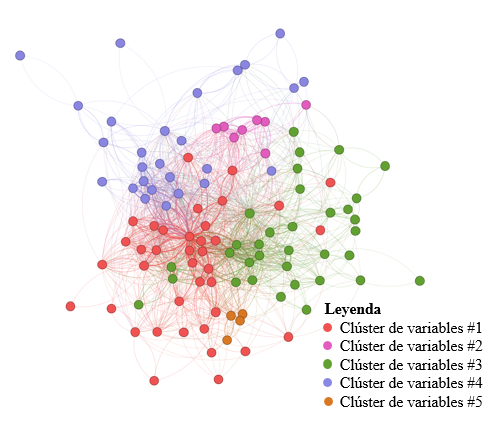
\includegraphics[width=8cm\textwidth]{mapa_correlaciones_con_leyenda.png} 
  \caption{Clustering de las 111 variables basado en correlaciones.}
  \label{fig:fig1}
\end{figure}

\subsection{Metodología}
El planteamiento del plan de acción está basado en tres aspectos de las características del dataset. A continuación se explica cada uno de ellos. 

En primer lugar, respecto de las variables de predicción, el dataset contiene once variables objetivo de naturaleza binaria y una variable categórica que puede tomar 7 categorías diferentes. Por ello, se puede tratar el problema tanto como uno de clasificación
con múltiples clases (multiclass) o múltiples etiquetas (multilabel). En tal medida, las clasificaciones de esta naturaleza se pueden abordar con los siguientes modelos
\begin{itemize}
    \item Regresión logística (Esquema One Vs. The Rest para el caso multiclass).
    \item Árboles de decisión.
    \item Redes neuronales.
    \item Modelos de gradient boosting (XGBoost, LightGBM).
\end{itemize}

En segundo lugar, las etiquetas están fuertemente sesgadas por la clase negativa. Para abordar este problema se considera probar cada una de las estrategias clásicas: subsampleo, \textit{k-folds} estratificado con validación cruzada, SMOTE y técnicas de \textit{boosting} para árboles de decisión. Adicionalmente, por esta misma razón se entrenará los modelos con las métricas de AUC-PR y F1-beta como objetivo. Esto debido a que se caracterizan por ser sensibles a la clase minoritaria valorando el desempeño de los modelos tanto sobre la clase negativa como positiva\cite{b?}. 

En tercer lugar, es necesario abordar la gran cantidad de valores faltantes en las 11 variables mencionadas previamente. Al respecto, los autores consultados coinciden con eliminar las variables que presentan excesiva cantidad de faltos, cada uno por distintos criterios. A nuestro criterio, se ha decidido probar primero un punto máximo de 30\% de faltos de acurdo con Govolenkin et. al. \cite{b1} y luego un punto de corte de 50\%, planteado por Narayan et. al. \cite{b??}.

Finalmente, se elegirá al mejor modelo  basado en la comparación de las métricas. Luego, este será sometido a una búsqueda en grilla para hallar los mejores parámetros.


\begin{thebibliography}{00}
\bibitem{b2} Ministerio de Salud del Perú-MINSA,``Muertes por infarto al miocardio-Perú,`` Dia mundial del Corazón, 2012. [En línea]. Disponible en: https://www.gob.pe/institucion/minsa/noticias/34838-al-ano-mas-de-4-mil-personas-mueren-por-infarto-en-el-peru.
\bibitem{b1}  S. E. Golovenkin et al.,``Trajectories, bifurcations, and pseudo-time in large clinical datasets: applications to myocardial infarction and diabetes data``, GigaScience, vol. 9, n.º 11. Oxford University Press (OUP), nov. 2020. doi: 10.1093/gigascience/giaa128.
\bibitem{e1} G. Quer, R. Arnaout, M. Henne, y R. Arnaout, ``Machine Learning and the Future of Cardiovascular Care: JACC State-of-the-Art Review``, J Am Coll Cardiol. 2021 Jan, 77 (3) 300–313. doi: 10.1016/j.jacc.2020.11.030
\bibitem{e2} J. Van den Eynde, M. Lachmann, K. Laugwitz, C. Manlhiot y S. Kutty, ``Successfully implemented artificial intelligence and machine learning applications in cardiology: State-of-the-art review``, Trends in Cardiovascular Medicine, Vol. 33, Issue 5, Pages 265-271, 2023. doi: 10.1016/j.tcm.2022.01.010.
\bibitem{e3} R. Sevakula, W. Au‐Yeung, J. Singh, E. Heist, E. Isselbacher y A. Armoundas, ``State‐of‐the‐Art Machine Learning Techniques Aiming to Improve Patient Outcomes Pertaining to the Cardiovascular System``, Journal of the American Heart Association. Vol. 9, Issue 4, 2020, Pages e013924. doi: 10.1161/JAHA.119.013924.
\bibitem{zz} H. Benzakour, C. Chekira, H. E. Fadili, y K. Zenkouar, ``A State of Art of Cardiovascular Diseases Using Machine Learning Algorithms``, 2023 7th IEEE Congress on Information Science and Technology (CiSt). IEEE, dic. 16, 2023. doi: 10.1109/cist56084.2023.10409886.
\bibitem{b??} Tiwari, R. (9 de febrero de 2023) ``Advanced Evaluation Metrics for Imbalanced Classification Models``. [En línea]. Disponible en: https://medium.com/cuenex/advanced-evaluation-metrics-for-imbalanced-classification-models-ee6f248c90ca
\bibitem{bp}  A. Moore y M. Bell, ``XGBoost, A Novel Explainable AI Technique, in the Prediction of Myocardial Infarction: A UK Biobank Cohort Study``, Clinical Medicine Insights: Cardiology, vol. 16. SAGE Publications, p. 117954682211336, ene. 2022. doi: 10.1177/11795468221133611.
\bibitem{ll} M. Mesinovic y K.-W. Yang, ``Multi-label Neural Model for Prediction of Myocardial Infarction Complications with Resampling and Explainability``, 2022 IEEE-EMBS International Conference on Biomedical and Health Informatics (BHI). IEEE, sep. 27, 2022. doi: 10.1109/bhi56158.2022.9926915.
\bibitem{by} A. Newaz, M. S. Mohosheu, y Md. A. Al Noman, ``Predicting complications of myocardial infarction within several hours of hospitalization using data mining techniques``, Informatics in Medicine Unlocked, vol. 42. Elsevier BV, p. 101361, 2023. doi: 10.1016/j.imu.2023.101361.
\bibitem{bx} D. A. Rossiev, S. E. Golovenkin, V. A. Shulman, y G. V. Matjushin, ``Neural networks for forecasting of myocardial infarction complications``, The Second International Symposium on Neuroinformatics and Neurocomputers. IEEE. doi: 10.1109/isninc.1995.480871.
\bibitem{bz} R. Ghafari et al., ``Prediction of the Fatal Acute Complications of Myocardial Infarction via Machine Learning Algorithms``, The Journal of Tehran University Heart Center. Knowledge E DMCC, ene. 30, 2024. doi: 10.18502/jthc.v18i4.14827.
\bibitem{b?} Narayan et. al. (2023) ``Myocardial Infarction Complications SDS322E - Final Project``. [En línea]. Disponible en: https://github.com/sarvagnyanarayan/myocardial-infarctions
\end{thebibliography} 
\end{document}
